\vspace{1cm}
\fancyhead[C]{\normalsize\textbf{$\qquad$ Teil I: Offene Aufgaben}}
\renewcommand{\labelenumi}{\theenumi.}
\section*{Aufgabe 1 (40 Punkte)}
\vspace{0.4cm}
\subsection*{\aufgabe{a}{12}}
Eine Rederei muss für ihre Schiffe Container herstellen, um darin Güter um die ganze Welt verschiffen zu können. Die Container müssen alle identisch sein und sollen, mathematisch formuliert, die Form eines Quaders  mit Länge $ x $, Höhe $ y $ und Breite $ z $ besitzen. Jeder Container muss ein Fassungsvermögen von 27 Volumeneinheiten haben. 
\begin{enumerate}
	\item[\textbf{(a1)}]
	Bestimmen Sie $ z $ als Funktion von $ x $ und $ y $ mithilfe der Volumenvorgabe jedes Containers.
	\item[\textbf{(a2)}] 
	Bestimmen Sie die Länge $ x $ und Höhe $ y $ (und damit die Breite $ z $ mit der Hilfe von Aufgabenteil (a1)), sodass die Container die minimale Oberfläche besitzen (und folglich die geringsten Herstellungskosten).
\end{enumerate}
\ \\
\textbf{Lösung:}
\begin{mdframed}
\underline{\textbf{Vorgehensweise:}}
\renewcommand{\labelenumi}{\theenumi.}
\begin{enumerate}
\item[\textbf{(a1)}] Stelle die Funktion mithilfe des Quadervolumens auf.
\item[\textbf{(a2)}] Verwende die Nebenbedingung für Oberfläche eines Quaders.
\end{enumerate}
\end{mdframed}
Die Verwendung von \glqq minimal\grqq \ lässt vermuten, dass ein Optimierungsproblem vorliegt.
Hierbei müssen wir zunächst prüfen ob und welche Nebenbedingungen vorliegen. Diese beschränken die Variablen. In unseren Fall müssen wir $ x $,  $ y $ und $ z $ so wählen, dass das Volumen des quaderförmigen Containers $ 27 $ Einheiten beträgt.
Es liegt also ein Minimierungsproblem mit Nebenbedingung vor.\\
\\
\underline{\textbf{(a1)} Stelle die Funktion mithilfe des Quadervolumens auf }\\
Ein Quader(Container) mit Länge $ x $, Höhe $ y $ und Breite $ z $ hat das Volumen $ V $
\begin{align*}
	V(x,y,z) = xyz.
\end{align*}
In unserem Fall soll das Volumen des Containers $ 27 $ Volumeneinheiten betragen.
Damit erhalten wir die Breite $ z $ als Funktion
\begin{align*}
	V(x,y,z) = xyz = 27  
	\ \Leftrightarrow \
	z(x,y) := z = \frac{27}{xy}
\end{align*}
für $ x,y > 0 $. Damit liegt eine Darstellung der Nebenbedingung in Abhängigkeit von $x$ und $y$ vor.\\
\\
\underline{\textbf{(a2)} Verwende die Nebenbedingung für Oberfläche eines Quaders}\\
Die Oberfläche eines Quaders(Containers) ist gegeben durch
\begin{align*}
	O(x,y,z) = 2 (xy + xz + yz).
\end{align*}
Diese soll nun unter der Nebenbedingung $V(x,y,z) = xyz = 27$ minimal werden. In der Teilaufgabe (a1) haben wir diese nach der Variablen $z$ umgeformt, wodurch diese in der Zielfunktion substituiert werden kann:
\begin{align*}
	F(x,y) = O(x,y,z(x,y))
	=
	2 ( xy +xz +yz )= 2 \left( xy + \frac{27}{y} + \frac{27}{x}\right)
	=
	2xy + \frac{54}{x} + \frac{54}{y}.
\end{align*}
Durch die Substitution liegt ein Extremwertproblem in zwei Variablen ohne Nebenbedingung vor um die Länge $x$, Höhe $y$ und Breite $z(x,y)$ für die minimale Oberfläche zu bestimmen.
Die partiellen Ableitungen erster Ordnung sind:
\begin{align*}
	F_x(x,y) &= 2 y - \frac{54}{x^2}\\
	F_y(x,y) &= 2 x - \frac{54}{y^2}.
\end{align*}
Die notwendige Bedingung für einen Extrempunkt in $(x_0,y_0)$ ist
\begin{align*}
	\textbf{(I)} &\ F_x(x_0,y_0) = 2 y_0 - \frac{54}{x_0^2} = 0
	\ \Leftrightarrow \
	= 2 y_0 x_0- \frac{54}{x_0} = 0\\
	\textbf{(II)} &\ F_y(x_0,y_0) = 2 x_0 - \frac{54}{y_0^2} = 0
	\ \Leftrightarrow \
	= 2 y_0 x_0- \frac{54}{y_0} = 0.
\end{align*}
Das Gleichsetzen von \textbf{(I)} und \textbf{(II)} liefert:
\begin{align*}
	2 y_0 x_0- \frac{54}{x_0} = 2 y_0 x_0- \frac{54}{y_0}
	\ \Leftrightarrow \
	 -\frac{54}{x_0} = -\frac{54}{y_0}
	 \ \Leftrightarrow \
	 \frac{1}{x_0} = \frac{1}{y_0}
	 \ \Leftrightarrow \
	 x_0 = y_0.
\end{align*}
Durch Einsetzen hiervon in \textbf{(I)} (oder \textbf{(II)}) erhalten wir:
\begin{align*}
	2x_0^2 - \frac{54}{x_0} = 0
	\ \Leftrightarrow \
	2 x_0^3 - 54 = 0
	\ \Leftrightarrow \
	2 x_0^3 = 54 
	\ \Leftrightarrow \
	x_0^3 = 27
	\ \Leftrightarrow \
	x_0 = \sqrt[3]{27} = 3.
\end{align*}
Damit gilt auch $y_0 = 3$ und es folgt 
\begin{align*}
	z(x_0,y_0) = \frac{27}{3 \cdot 3 } = 3.
\end{align*}
Somit liegt die potientiell minimale Fläche für die Länge, Höhe und Breite von $3$ vor.\\
\\
Um zu zeigen, dass an $(x_0,y_0) =(3,3)$ wirklich ein Minimum vorliegt, muss die hinreichende Bedingung
\begin{align*}
	\Delta(x_0,y_0)
	=F_{xx}(x_0,y_0)F_{yy}(x_0,y_0)
	- (F_{xy}(x_0,y_0))^2 > 0 
\end{align*}
mit $F_{xx}(x_0,y_0) > 0 $ und $F_{yy}(x_0,y_0)>0$ erfüllt sein.
Für die Ableitungen zweiter Ordnung gilt:
\begin{align*}
	F_{xx}(x,y)
	=
	\frac{2 \cdot 54}{x_3}, 
	\quad
	F_{yy}(x,y)
	=
	\frac{2 \cdot 54}{y_3},
	\quad
	F_{xy}(x,y)
	=
	F_{yx}(x,y) = 2.
\end{align*}
Durch Einsetzen von $(x_0,y_0)$ erhalten wir
\begin{align*}
	F_{xx}(3,3) = F_{yy}(3,3) = \frac{2 \cdot 54}{27} = 2 \cdot 2 = 4 > 0
\end{align*}
und es folgt:
\begin{align*}
	\Delta(3,3) = 4^2 - 2^2 = 12 > 0.
\end{align*}
Damit liegt für $(x_0,y_0) = (3,3)$ wirklich ein Minimum von $F$ vor, d.h. der Container hat die minimale Oberfläche als Würfel mit der Kantenlänge $3$.

\newpage

\subsection*{\aufgabe{b}{14}}
Die Renditen der Aktien der Unternehmen BEST, SUCCESS und WINNER hängen von einem von vier möglichen Szenarien ab, wie sich die Finanzmärkte entwickeln. Die möglichen Szenarien und Renditen der jeweiligen Aktie werden in folgender Tabelle beschrieben:
\begin{table}[H]
	\centering
	%
	\begin{tabular}{c c c c}
		\hline
		Szenario & BEST  &  SUCCESS &  WINNER \\ 
		\hline
		$ s_1 $ & $ 3 $ & $ 1 $ & $ 2 $  \\ 
		$ s_2 $ & $ 2 $ & $ 2 $ & $ 2 $ \\
		$ s_3 $ & $ 3 $ & $ 3 $ & $ 1 $ \\
		$ s_4 $ & $ -1 $ & $ 1 $ & $ 0 $\\
		\hline
	\end{tabular}%
\end{table}
Eine Investorin möchte in die drei Aktien investieren. Ihr Ziel ist es folgende Rendite, abhängig vom jeweiligen Szenario, zu generieren:
\begin{table}[H]
	\centering
	%
	\begin{tabular}{c c}
		\hline
		Szenario & Rendite  \\
		\hline
		$ s_1 $ & $ 5 $ \\ 
		$ s_2 $ & $ 3 $  \\
		$ s_3 $ & $ a $  \\
		$ s_4 $ & $ -2 $ \\
		\hline
	\end{tabular}%
\end{table}
wobei $ a \in \mathbb{R} $.
\begin{enumerate}
	\item[\textbf{(b1)}]
	Bestimmen Sie das lineare Gleichungssystem, welches das Allokationsproblem der Investorin beschreibt.
\end{enumerate}
Verwenden Sie den Gauß-Algorithmus für die folgenden Aufgaben.
\begin{enumerate}
	\item[\textbf{(b2)}] 
	Für welche Werte von $ a $ existiert eine Lösung des Investitionsproblems?
	\item[\textbf{(b3)}]
	Bestimmen Sie für $ a \ = \ -3.5 $ die Investitionsstrategie der Investorin, welche die entsprechenden Renditen je nach Szenario erwirtschaftet.
\end{enumerate}
\ \\
\textbf{Lösung:}
\begin{mdframed}
\underline{\textbf{Vorgehensweise:}}
\renewcommand{\labelenumi}{\theenumi.}
\begin{enumerate}
\item[\textbf{(b1)}] Stelle das lineare Gleichungssystem auf.
\item[\textbf{(b2)}] 
\begin{enumerate}
	\item[1.] Wende das elementare Zeilenumformungen an (Gauß-Verfahren).
	\item[2.] Überlege ob Lösungen existieren und prüfe deren Eindeutigkeit.
\end{enumerate}

\item[\textbf{(b3)}] Löse das LGS für $a=-3.5 $.
\end{enumerate}
\end{mdframed}

In dieser Aufgabe liegt ein lineares Gleichungssystem vor.
Dies müssen wir zunächst aus der Aufgabenstellung extrahieren und darauf dessen Struktur und Eigenschaften untersuchen.
Wir schreiben die Renditen der einzelnen Szenarien zu einer Aktie als Vektor und linear kombinieren diese zu den Gesamtrenditen der einzelnen Szenarien:
\begin{align*}
	x_1
	\begin{pmatrix}
		3 \\ 2 \\ 3 \\ -1
	\end{pmatrix}
	+
	x_2
	\begin{pmatrix}
		1 \\ 2 \\ 3 \\ 1
	\end{pmatrix}
	+
	x_3
	\begin{pmatrix}
		2 \\ 2 \\ 1 \\ 0
	\end{pmatrix}
	=
	\begin{pmatrix}
		5 \\ 3 \\ a \\ -2
	\end{pmatrix}
\end{align*}

\underline{\textbf{(b1)} Stelle das lineare Gleichungssystem auf}\\
In der Einleitung haben wir das Aufstellen des Gleichungssystems
\begin{align*}
	s_1 : 3x_1 +  \ x_2 + 2 x_3 \ &=\ 5\\
	s_2 : 2x_2 + 2 x_2 + 2 x_3 \ &= \ 3\\
	s_3 : 3x_1 + 3x_2 + \ \ x_3 \ &= \ a \ \\
	s_4 : -x_1 + x_2 \qquad \quad \ \ &= -2
\end{align*}
für die einzelen Szenarien $s_i$ mit $i = 1,...,4$ vorwegenommen.
Übersetzt in eine erweiterte Koeffizientenmatrix erhalten wir:
\begin{align*}
	(A,\mathbf{b})
	=
	\begin{pmatrix}
		3 & 1 & 2 & \BAR & 5\\
		2 & 2 & 2 & \BAR & 3\\
		3 & 3 & 1 & \BAR & a \\
		-1 & 1 & 0 & \BAR & -2
	\end{pmatrix}.
\end{align*}
\ \\
\underline{\textbf{(b2)} 1. Wende das elementare Zeilenumformungen an (Gauß-Verfahren)}\\
Durch elementare Zeilenumformungen erhalten wir:
\begin{align*}
	\begin{gmatrix}[p]
		3 & 1 & 2 & \BAR & 5\\
		2 & 2 & 2 & \BAR & 3\\
		3 & 3 & 1 & \BAR & a \\
		-1 & 1 & 0 & \BAR & -2
		\rowops
		\add[ \cdot 3]{3}{2}
		\add[ \cdot 2]{3}{1}
		\add[ \cdot 3]{3}{0}
	\end{gmatrix}
	&\leadsto
	\begin{gmatrix}[p]
		0 & 4 & 2 & \BAR & -1\\
		0 & 4 & 2 & \BAR & -1\\
		0 & 6 & 1 & \BAR & a - 6\\
		-1 & 1 & 0 & \BAR & -2
		\rowops
		\add[ \cdot (-1)]{0}{2}
	\end{gmatrix}
	\leadsto
	\begin{gmatrix}[p]
		0 & 4 & 2 & \BAR & -1\\
		0 & 0 & 0 & \BAR & 0\\
		0 & 6 & 1 & \BAR & a - 6\\
		-1 & 1 & 0 & \BAR & -2
	\end{gmatrix}\\
	&\leadsto
	\begin{gmatrix}[p]
		-1 & 1 & 0 & \BAR & -2\\
		0 & 4 & 2 & \BAR & -1\\
		0 & 6 & 1 & \BAR & a - 6\\
		0 & 0 & 0 & \BAR & 0
		\rowops
		\mult{1}{ \cdot (3)}
		\mult{2}{ \cdot (2)}
	\end{gmatrix}
	\leadsto
	\begin{gmatrix}[p]
		-1 & 1 & 0 & \BAR & -2\\
		0 & 12 & 6 & \BAR & -3\\
		0 & 12 & 2 & \BAR & 2a - 12\\
		0 & 0 & 0 & \BAR & 0
		\rowops
		\mult{1}{ \cdot (3)}
		\mult{2}{ \cdot (2)}
	\end{gmatrix}\\
	&\leadsto
	\begin{gmatrix}[p]
		-1 & 1 & 0 & \BAR & -2\\
		0 & 12 & 6 & \BAR & -3\\
		0 & 12 & 2 & \BAR & 2a - 12\\
		0 & 0 & 0 & \BAR & 0
		\rowops
		\add[ \cdot (-1)]{1}{2}
	\end{gmatrix}
	\leadsto
	\begin{gmatrix}[p]
		-1 & 1 & 0 & \BAR & -2\\
		0 & 12 & 6 & \BAR & -3\\
		0 & 0 & 4 & \BAR & 2a - 9\\
		0 & 0 & 0 & \BAR & 0
		\rowops
		\mult{1}{ \cdot (\frac{1}{3})}
	\end{gmatrix}\\
	&\leadsto
	\begin{gmatrix}[p]
		-1 & 1 & 0 & \BAR & -2\\
		0 & 4 & 2 & \BAR & -1\\
		0 & 0 & -4 & \BAR & 2a - 9\\
		0 & 0 & 0 & \BAR & 0
	\end{gmatrix}
\end{align*}
\ \\
\underline{\textbf{(b2)} 2. Überlege ob Lösungen existieren und prüfe deren Eindeutigkeit}\\
Damit ein Gleichungssystem $ A \mathbf{x} = \mathbf{b} $ mindestens eine Lösung besitzt, muss $ \mathrm{rg}(A) = \mathrm{rg}( A,\mathbf{b} ) $ gelten.
Mit $n$ bezeichnen wir die Anzahl der Unbekannten.
Falls mindestens eine Lösung existiert, können zwei Fälle eintreten:
\begin{description}
	\item[Fall 1 $\mathbf{\mathrm{rg}(A) = \mathrm{rg}(A,b) = n}$:] Es existiert genau eine (eindeutige) Lösung.
	\item[Fall 2 $\mathbf{\mathrm{rg}(A) = \mathrm{rg}(A,b) < n }$:] Es existieren unendlich viele Lösungen.
\end{description}
In unserem Fall gilt unabhängig von $a$ $\mathrm{rg}(A) = \mathrm{rg}(A,\mathbf{b}) = 3 = n$. Damit existiert für alle $a \in \mathbb{R}$ eine eindeutige Lösung für das Investitionsproblem.\\
\\
\underline{\textbf{(b3)} Löse das LGS für $a=-3.5 $}\\
Wir setzen $a = -3.5 = - \frac{7	}{2}$ in die erweiterte Koeffizientenmatrix ein und erhalten durch elementare Zeilenumformungen:
\begin{align*}
	\begin{gmatrix}[p]
		-1 & 1 & 0 & \BAR & -2\\
		0 & 4 & 2 & \BAR & -1\\
		0 & 0 & -4 & \BAR & -16\\
		0 & 0 & 0 & \BAR & 0
		\rowops
		\mult{2}{ \cdot (\frac{1}{4})}
	\end{gmatrix}
	&\leadsto
	\begin{gmatrix}[p]
		-1 & 1 & 0 & \BAR & -2\\
		0 & 4 & 2 & \BAR & -1\\
		0 & 0 & -1 & \BAR & -4\\
		0 & 0 & 0 & \BAR & 0
		\rowops
		\add[ \cdot 2]{2}{1}
		\mult{0}{ \cdot 4}
	\end{gmatrix}
	\leadsto
	\begin{gmatrix}[p]
		-4 & 4 & 0 & \BAR & -8\\
		0 & 4 & 0 & \BAR & -9\\
		0 & 0 & 1 & \BAR & 4\\
		0 & 0 & 0 & \BAR & 0
		\rowops
		\add[ \cdot (-1)]{1}{0}
		\mult{2}{ \cdot (-1)}
	\end{gmatrix}\\
	&\leadsto
	\begin{gmatrix}[p]
		-4 & 0 & 0 & \BAR & 1\\
		0 & 4 & 0 & \BAR & -9\\
		0 & 0 & 1 & \BAR & 4\\
		0 & 0 & 0 & \BAR & 0
		\rowops
		\mult{0}{ \cdot (-\frac{1}{4})}
		\mult{1}{ \cdot \frac{1}{4}}
	\end{gmatrix}
	\leadsto
	\begin{gmatrix}[p]
		1 & 0 & 0 & \BAR & -\frac{1}{4}\\
		0 & 1 & 0 & \BAR & - \frac{9}{4}\\
		0 & 0 & 1 & \BAR & 4\\
		0 & 0 & 0 & \BAR & 0
	\end{gmatrix}.
\end{align*}
Hieran lässt sich die Lösung 
\begin{align*}
	x_1 = - \frac{1}{4} = - 0.25, \quad
	x_2 = -\frac{9}{4} = - 2.25, \quad
	x_3 = 4
\end{align*}
direkt ablesen.\\
\\
Alternativ lässt sich die obere Dreiecksform nach den elementaren Zeilenumformungen ausnutzen. Die erweiterte Koeffizientenmatrix
\begin{align*}
	\begin{gmatrix}[p]
		-1 & 1 & 0 & \BAR & -2\\
		0 & 4 & 2 & \BAR & -1\\
		0 & 0 & -4 & \BAR & -16\\
		0 & 0 & 0 & \BAR & 0
	\end{gmatrix}
	&\leadsto
	\begin{gmatrix}[p]
		-1 & 1 & 0 & \BAR & -2\\
		0 & 4 & 2 & \BAR & -1\\
		0 & 0 & 1 & \BAR & 4\\
		0 & 0 & 0 & \BAR & 0
	\end{gmatrix}
\end{align*}
enthält die Gleichungen:
\begin{align*}
	-x_1 + x_2 &= -2 \\
	4 x_2 + 2 x_3 &= 1 \\
	x_3 &= 4.
\end{align*}
Durch Rückwärtseinsetzen erhalten wir ebenso die Lösung.
\newpage
\subsection*{\aufgabe{c}{14}}
Ein Konsument deckt seine Nachfrage nach zwei Gütern. Dabei beschreibt $ c_1 $ die Menge von Gut $ 1 $ und $ c_2 $ die Menge von Gut $ 2 $. Der Konsument besitzt die Nutzenfunktion $ u(c_1,c_2) $, welche als Kehrwert der geometrischen Distanz zwischen dem Konsumbündel $ (c_1,c_2) $ und einem angestrebten Konsumbündel $ (3,3) $ definiert ist. Der Preis für Gut $ 1 $ beträgt $ p_1 \ = \ 2 $ (CHF) und für Gut $ 2 $ $ p_2 \ = \ 3 $ (CHF). Der Konsument besitzt das Einkommen von $ e = 10 $ (CHF).
\begin{enumerate}
	\item[\textbf{(c1)}] 
	Bestimmen Sie die Nutzenfunktion des Konsumenten sowie dessen Budgetrestriktion.
	\item[\textbf{(c2)}]
	Vereinfachen Sie das Optimierungsproblem, indem Sie es geeignet transformieren und bestimmen Sie das optimale Konsumbündel für den Konsumenten.
\end{enumerate}
\ \\
\textit{Bemerkungen: Der Kehrwert eines mathematischen Ausdrucks $ x $ ist definiert als $ \frac{1}{x} $. Es ist \textbf{nicht} nötig zu zeigen, dass es sich um ein Maximum handelt.}
\\ \\
\textbf{Lösung:}
\begin{mdframed}
\underline{\textbf{Vorgehensweise:}}
\begin{enumerate}
\item[\textbf{(c1)}] Stelle Nutzenfunktion sowie die Budgetrestrikton(Nebenbedingung) auf.
\item[\textbf{(c2)}]
\begin{enumerate}
	\item[1.] Transformiere die Zielfunktion.
	\item[2.] Löse die Aufgabe mit der Lagrange-Methode.
	\item[3.] Löse die Aufgabe durch Substitution.
\end{enumerate}
\end{enumerate}
\end{mdframed}

Diese Aufgabe ist ein Optimierungsproblem mit Nebenbedigung.
Da der Konsument ein Einkommen von $10$ (CHF) zur Verfügung hat kann er mit den Gütern 1 und 2  die Nutzenfunktion nicht beliebig maximieren, d.h. gesucht ist das Maximum der Nutzenfunktion $u(c_1,c_2)$ unter der Einkommensrestriktion von $10$ (CHF).\\
\\
\underline{\textbf{(c1)} Stelle Nutzenfunktion sowie die Budgetrestrikton(Nebenbedingung) auf}\\
Die geometrische Distanz zweier Punkte $(x_1,y_1)$ und $(x_2,y_2)$ ist gegeben durch
\begin{align*}
	\left|(x_1,y_1) - (x_2,y_2) \right|
	=
	\sqrt{(x_1 -x_2)^2 + (y_1-y_2)^2}. 
\end{align*}
Die Nutzenfunktion ist die Zielfunktion der Optimierung.Nach der Aufgabenstellung ist diese der Kehrwert des geometrischen Abstandes der Konsumbündel $(c_1,c_2)$ und $(3,3)$, d.h.:
\begin{align*}
	u(c_1,c_2)
	=
	\frac{1}{\left|(c_1,c_2) - (3,3) \right|}
	=
	\frac{1}{\sqrt{(c_1 -3)^2 + (c_2-3)^2}}.
\end{align*}
Die Budgetrestriktion(Nebenbedingung) ist gegeben durch
\begin{align*}
	p_1 c_1 + p_2 c_2= e 
	\ \Rightarrow \
	2 c_1 + 3 c_2 = 10
	\ \Leftrightarrow \
	\varphi(c_1,c_2) = 2 c_1 + 3c_3 - 10= 0.
\end{align*} 
\  \\
\underline{\textbf{(c2)} 1. Transformiere die Zielfunktion}\\
Das Optimierungsproblem mit Nebenbedingung liegt in der Form 
\begin{align*}
	\max \limits_{c_1,c_2} u(c_1,c_2)
	=
	\max \limits_{c_1,c_2} \frac{1}{\sqrt{(c_1 -3)^2 + (c_2-3)^2}}
	, \qquad \varphi(c_1,c_2) = 2 c_1 + 3c_3 - 10= 0
\end{align*}
vor. Die Zielfunktion können wir hierbei durch mehrere Transformationen vereinfachen. Die Funktion $\frac{1}{x}$ ist streng monoton fallend, d.h. die Zielfunktion erreicht ihr Maximum, sobald der Nenner minimal wird. Die erste Transformation erreichen wir, indem wir das Minimum des Nenners suchen:
\begin{align*}
	\min \limits_{c_1,c_2}
	\hat{u}(c_1,c_2)
	=
	\min \limits_{c_1,c_2} \sqrt{(c_1 -3)^2 + (c_2-3)^2}
	, \qquad \varphi(c_1,c_2) = 2 c_1 + 3c_2 - 10= 0.
\end{align*}
Die Wurzelfunktion ist streng monoton wachsend, d.h. sie erhält das Minimum. Deswegen können wir die Wurzelfunktion ignorieren und erhalten als endgültige Optimierungsproblem:
\begin{align*}
	\min \limits_{c_1,c_2}
	\tilde{u}(c_1,c_2)
	=
	\min \limits_{c_1,c_2} (c_1 -3)^2 + (c_2-3)^2
	, \qquad \varphi(c_1,c_2) = 2 c_1 + 3c_2 - 10= 0.
\end{align*}
Dieses können wir mit dem Verfahren der Wahl lösen (Lagrange oder Substitution).\\
\\
\underline{\textbf{(c2)} 1. Löse die Aufgabe mit der Lagrange-Methode}\\
Mit unserern Transformationen erhalten wir die Lagrange-Funktion:
\begin{align*}
	L(c_1,c_2,\lambda)
	=
	\tilde{u}(c_1,c_2) + \lambda \varphi(c_1,c_2)
	=
	(c_1-3)^2 + (c_2-3)^2 + \lambda ( 2c_1 + 3 c_2 -10).
\end{align*}
Die partiellen Ableitungen sind gegeben durch:
\begin{align*}
	\frac{\partial L}{\partial c_1}(c_1, c_2 , \lambda)
	&= 2(c_1 -3) + 2 \lambda\\
	\frac{\partial L}{\partial c_2}(c_1, c_2 , \lambda)
	&= 2(c_2 -3) + 3 \lambda \\
	\frac{\partial L}{\partial \lambda}(c_1, c_2 , \lambda)
	&= 2 c_1 + 3 c_2 - 10 .
\end{align*}
Damit ergeben sich die Lagrange-Bedingungen:
\begin{align*}
	\text{(I)} &\ 2(c_1 -3) + 2 \lambda = 0 
	\ \Rightarrow \
	\lambda = - c_1 + 3	\\
	\text{(II)} &\ 2(c_2 -3) + 3 \lambda  = 0
	\ \Rightarrow \
	\lambda = - \frac{2}{3} c_2 + 2
	\\
	\text{(III)} &\ 2 c_1 + 3 c_2 - 10 = 0.
\end{align*}
Das Gleichsetzen von (I) und (II) ergibt
\begin{align*}
	-c_1 + 3 = - \frac{2}{3} c_2 +2
	\ \Leftrightarrow \
	c_1 = \frac{2}{3} c_2 +1 \quad (\ast) .
\end{align*}
Einsetzen hiervon in (III) liefert:
\begin{align*}
	2 \left(\frac{2}{3}c_2 + 1\right) + 3 c_2 - 10 = 0
	\ \Leftrightarrow \
	\frac{4}{3} c_2 + \frac{9 }{3} c_2 = \frac{13}{3} c_2 = 8 
	\ \Leftrightarrow \
	&c_2 = \frac{24}{13}\\ 
	\
	\overset{(\ast)}{\Rightarrow}
	&c_1 = \frac{2}{3} \cdot\frac{24}{13} + 1
	= \frac{16}{13} + \frac{13}{13} = \frac{29}{13}.
\end{align*}
Das optimale Konsumbündel ist (vermutlich) durch
\begin{align*}
	c_1^\star = \frac{29}{13}, \qquad 
	c_2^\star = \frac{24}{13}.
\end{align*}
gegeben. Mithilfe der Lagrange-Methode haben wir jedoch nur eine notwendige Bedingung für eine Extremstelle unter einer Nebenbedingung.
Die transformierte Zielfunktion ist ein nach oben geöffnetes Paraboloid und die Nebenbedingung ist eine Gerade.
Unabhängig davon wie wir eine Gerade (die Nebenbedingung) durch das Paraboloid legen hat, finden wir immer ein Minimum wenn die Gerade auf dem Paraboloid ablaufen.
\newpage
In unserem Fall können wir das durch die Grafik
\begin{center}
	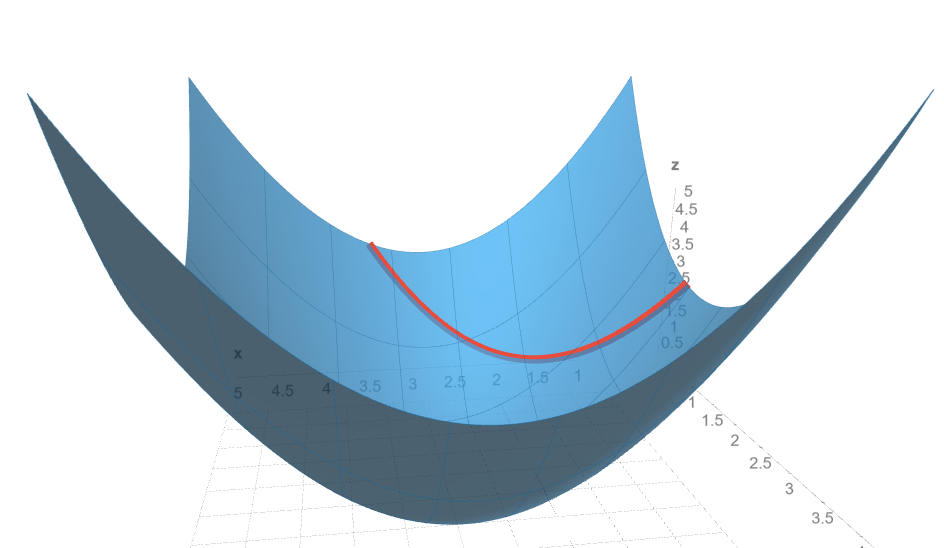
\includegraphics[width=0.6\textwidth]{pictures/aufgabe1_c}
\end{center}
veranschaulichen.
Hierbei ist die rote Linie die Budgetrestriktion auf der transformierten Zielfunktion.\\
\\
\underline{\textbf{(c2)} 3. Löse die Aufgabe durch Substitution}\\
Um die Aufgabe durch Substitution zu lösen, formen wir die Budgetrrestriktion nach einer der beiden Variablen um:
\begin{align*}
	2 c_1 + 3 c_2 = 10
	\ \Leftrightarrow \ 
	2c_1 = 10 - 3 c_2 
	\ \Leftrightarrow \
	c_1 = 5 - \frac{3}{2} c_2.
\end{align*}
Wenn wir dies in die Zielfunktion erhalten wir mit
\begin{align*}
	F(c_2)
	&:= 
	\tilde{u}\left(5 - \frac{3}{2} c_2, c_2\right)
	= 
	\left(5 - \frac{3}{2} c_2 -3 \right)^2 + (c_2 -3 )^2
	=
	\left(2 - \frac{3}{2} c_2\right)^2 + (c_2 -3)^2\\
	&=
	\frac{9}{4} \left(\frac{4}{3} - c_2\right)^2 + (c_2 -3)^2
	=
	\frac{9}{4} \left(c_2 -\frac{4}{3} \right)^2 + (c_2 -3)^2.
\end{align*}
Die Ableitung erster Ordnung ist gegeben durch:
\begin{align*}
	F^\prime(c_2)
	=
	\frac{9}{2} \left(c_2 - \frac{4}{3}\right) + 2 (c_2 -3)
	=
	\frac{9}{2} c_2 - 6 + 2 c_2 - 6
	=
	\frac{13}{2} c_2 -12.
\end{align*}
Die notwendie Bedingung für ein Minimum in $c^\star_2$ ist
\begin{align*}
	F^\prime(c_2^\star) = 0 
	\ \Leftrightarrow \
	\frac{13}{2} c_2^\star - 12 = 0  
	\ \Leftrightarrow \
	\frac{13}{2} c_2^\star = 12 
	\ \Leftrightarrow \
	c_2^\star = \frac{24}{13}
\end{align*}
und mit der Rücksubstitution erhalten wir:
\begin{align*}
	c_1^\star = 5 - \frac{3}{2} \cdot \frac{24}{13}
	= \frac{29}{13}.
\end{align*}
Wegen 
\begin{align*}
	F^{\prime \prime}(c_2^\star ) = \frac{13}{2} > 0
\end{align*}
liegt an dem Konsumbündel $(c^\star_1,c^\star_2)$ ein Minimum von $\tilde{u}$ bzw. Maximum von $u$ unter der Budgetrestriktion vor.


\newpage

